\hsection{Relationships of a Higher Degree}%
%
\begin{figure}%
\centering%
%
\subfloat[][%
A reproduction of \cref{fig:erdStudentModuleProf3}, which illustrates a ternary relationship of students, modules, and professors with the relationship attribute semester. %
This graphic was painted using \yEd.%
\label{fig:erdStudentModuleProf3B}%
]{\includegraphics[width=0.9\linewidth]{\erdStudentModuleProfIII}}%
%
\floatRowSep%
%
\subfloat[][%
One possible transformation of \cref{fig:erdStudentModuleProf3} to a logical model using \pgmodeler.%
\label{fig:logicalStudentModuleProf}%
]{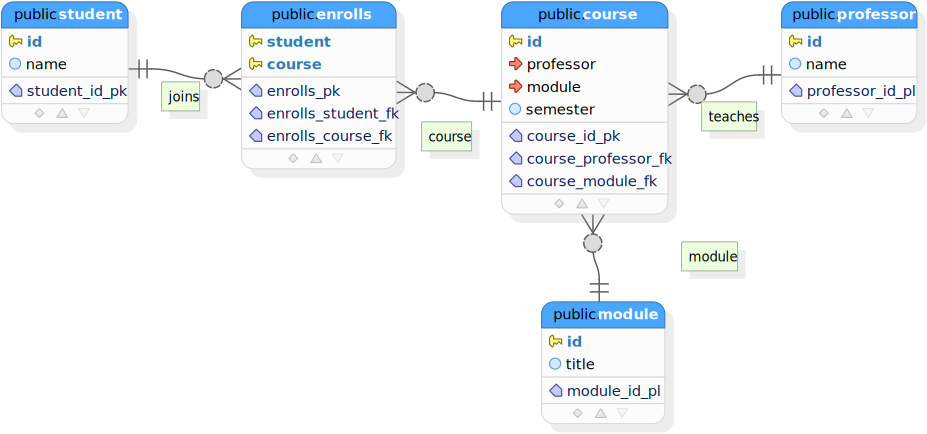
\includegraphics[width=0.97\linewidth]{\currentDir/logicalStudentModuleProf}}%
%
\caption{The representation of relationships with a degree higher than two in relational logical models.}%
\label{fig:logicalStudentModuleProfII}%
\end{figure}%
%
In \cref{fig:erdStudentModuleProf3B}, we reproduce a figure from \dref{sec:conceptual:relationships} where a ternary relationship is illustrated.
The entity types \emph{Professor}, \emph{Student}, and \emph{Module} are related with each other and this relationship even has a relationship attribute.
The professor teaches a module in a certain semester.
The student enrolls in that taught module in that semester.

We now want to create a logical model that fits to this scenario.
First we sort out the easy things.
The entity types become tables with surrogate primary keys.
We thus get the tables \sqlil{module}, \sqlil{professor}, and \sqlil{student}.
In order to add a bit more sense to this example, we include the attribute \sqlil{name} in the tables \sqlil{student} and \sqlil{professor} as well as \sqlil{title} in \sqlil{module}.

We then construct the ternary relationship.
We basically have two choices to do this:%
%
\begin{enumerate}%
%
\item We can create one single table \sqlil{takes_place}.
It will have three foreign keys to the tables \sqlil{professor}, \sqlil{student}, and \sqlil{module}, as well as a column~\sqlil{semester}. %
It will store all the data and participants of the ternary relationship.%
%
\item We can create one table~\sqlil{course} with a surrogate key and use it to store the \inQuotes{module-instantiation}. %
An instantiation is a module being taught by a professor in one semester. %
This table thus will have foreign keys to the tables \sqlil{professor} and \sqlil{module} as well as the column~\sqlil{semester}. %
We then create a second table~\sqlil{enrolls} that has two foreign keys, one for the table~\sqlil{student} and one for the table~\sqlil{course}. %
It stores the \inQuotes{enrolls} relationship of students towards module-instatiations.%
%
\end{enumerate}%
%
Both choices would be feasible, but we go with the second one.
The idea is that we can also consider the realization of a module by a certain professor in a semester as an entity in its own right.
This entity would have the attribute \sqlil{semester}, but could also have arbitrary other attributes that we may want to add later.
Relating the students to that \sqlil{course} table by using a separate table then makes sense.

This approach has two striking benefits.
First, it avoids avoids redundancy.
The first idea, namely storing the student, module, and professor keys in a single table, would mean that we store the fact that \inQuotes{Prof.~Mrs.~Bibba} teaches~\inQuotes{Mathematics~101} again and again.
By using two tables, one for module instances and one for module enrollment, we only store it once.

Second, this second method can properly represent a situation in which a professor teaches the same module twice in one semester.
Due to limited room capacity or scheduling conflicts of student time tables, it might indeed possible that \inQuotes{Prof.~Mrs.~Bibba} teaches~\inQuotes{Mathematics~101} on Mondays for one group of students and on Tuesdays for a second group.
In the first solution, there is no way to express this fact.
In the second one, which we chose, we can simply instantiate the module twice.

Anyway, once we made up our mind, we can create the model.
We do this using, of course, \pgmodeler\ and get the logical schema illustrated in \cref{fig:logicalStudentModuleProf}.

\gitLoadAndExecSQL{teaching_1:01_teaching_database_database_2001}{}{teachingManagement/logical/teaching_database_1/generated_sql}{01_teaching_database_database_2001.sql}{}{}{}%
\listingSQL{teaching_1:01_teaching_database_database_2001}{The generated script to create the \sqlil{teaching_database}~\db.}%
%
\gitLoadAndExecSQL{teaching_1:03_public_student_table_5071}{}{teachingManagement/logical/teaching_database_1/generated_sql}{03_public_student_table_5071.sql}{teaching_database}{}{}%
\listingSQL{teaching_1:03_public_student_table_5071}{The generated script to create the table~\sqlil{student}.}%
%
\gitLoadAndExecSQL{teaching_1:04_public_professor_table_5087}{}{teachingManagement/logical/teaching_database_1/generated_sql}{04_public_professor_table_5087.sql}{teaching_database}{}{}%
\listingSQL{teaching_1:04_public_professor_table_5087}{The generated script to create the table~\sqlil{professor}.}%
%
\gitLoadAndExecSQL{teaching_1:05_public_module_table_5095}{}{teachingManagement/logical/teaching_database_1/generated_sql}{05_public_module_table_5095.sql}{teaching_database}{}{}%
\listingSQL{teaching_1:05_public_module_table_5095}{The generated script to create the table~\sqlil{module}.}%
%
\gitLoadAndExecSQL{teaching_1:06_public_course_table_5105}{}{teachingManagement/logical/teaching_database_1/generated_sql}{06_public_course_table_5105.sql}{teaching_database}{}{}%
\listingSQL{teaching_1:06_public_course_table_5105}{The generated script to create the table~\sqlil{course} which relates the tables~\sqlil{professor} and~\sqlil{module}.}%
%
\gitLoadAndExecSQL{teaching_1:07_public_enrolls_table_5131}{}{teachingManagement/logical/teaching_database_1/generated_sql}{07_public_enrolls_table_5131.sql}{teaching_database}{}{}%
\listingSQL{teaching_1:07_public_enrolls_table_5131}{The generated script to create the table~\sqlil{enrolls} which relates the tables~\sqlil{student} and~\sqlil{course}.}%
%
\gitLoadAndExecSQL{teaching_1:08_public_course_course_professor_fk_constraint_5116}{}{teachingManagement/logical/teaching_database_1/generated_sql}{08_public_course_course_professor_fk_constraint_5116.sql}{teaching_database}{}{}%
\listingSQL{teaching_1:08_public_course_course_professor_fk_constraint_5116}{The generated script to create the constraint enforcing that each row in table~\sqlil{course} is related to exactly one row in table~\sqlil{professor}.}%
%
\gitLoadAndExecSQL{teaching_1:09_public_course_course_module_fk_constraint_5117}{}{teachingManagement/logical/teaching_database_1/generated_sql}{09_public_course_course_module_fk_constraint_5117.sql}{teaching_database}{}{}%
\listingSQL{teaching_1:09_public_course_course_module_fk_constraint_5117}{The generated script to create the constraint enforcing that each row in table~\sqlil{course} is related to exactly one row in table~\sqlil{module}.}%
%
\gitLoadAndExecSQL{teaching_1:10_public_enrolls_enrolls_student_fk_constraint_5145}{}{teachingManagement/logical/teaching_database_1/generated_sql}{10_public_enrolls_enrolls_student_fk_constraint_5145.sql}{teaching_database}{}{}%
\listingSQL{teaching_1:10_public_enrolls_enrolls_student_fk_constraint_5145}{The generated script to create the constraint enforcing that each row in table~\sqlil{enrolls} is related to exactly one row in table~\sqlil{student}.}%
%
\gitLoadAndExecSQL{teaching_1:11_public_enrolls_enrolls_course_fk_constraint_5151}{}{teachingManagement/logical/teaching_database_1/generated_sql}{11_public_enrolls_enrolls_course_fk_constraint_5151.sql}{teaching_database}{}{}%
\listingSQL{teaching_1:11_public_enrolls_enrolls_course_fk_constraint_5151}{The generated script to create the constraint enforcing that each row in table~\sqlil{enrolls} is related to exactly one row in table~\sqlil{course}.}%
%
\gitLoadAndExecSQL{teaching_database_1:insert_and_select}{}{teachingManagement/logical/teaching_database_1}{insert_and_select.sql}{teaching_database}{}{}%
\listingSQLandOutput{teaching_database_1:insert_and_select}{%
Inserting into and selecting data from the tables in the \sqlil{teaching_database}.%
}{}%
%
\gitExecSQLraw{}{}{teachingManagement/logical/teaching_database_1}{cleanup.sql}{}{}{}%
%

For this purpose, we extend the model further with reasonable assumptions about cardinalities and modalities.
For example, it makes sense to assume that each row in table~\sqlil{course} must be related to exactly one row in table~\sqlil{professor} and exactly one row in table~\sqlil{module}.
We do not permit a course that represents no module of the curriculum and we also do not permit a course that teaches the knowledge of multiple modules at once.
Similarly, we cannot have a course without professor and also we do not permit more than one professor to teach a course.
Well, the latter may actually be possible.
Maybe that would be a good question to bring up during the requirements gathering process or later during conceptual modelling when sitting down with our stakeholders in the university.
At least for now, we do not permit that~(as it would also make our relationship patterns more complicated).

Professors can teach multiple modules and each module can be taught by multiple professors.
We \emph{could} add a \sqlilIdx{UNIQUE} constraint over the combination of the columns~\sqlil{module}, \sqlil{professor}, and~\sqlil{semester}.
This would mean that a professor cannot teach the same module twice in the same semester.
Then again, we can also permit this.
We can easily imagine some \inQuotes{service modules,} like \inQuotes{Mathematics for Engineers,} that many be offered by the School of Mathematics to several other schools, say the School of Computer Science, the School the Engineering, and the School of Agriculture.
Then a professor may offer the same module several times in the same semester, just for different student groups.

We also enforce that each record in the table~\sqlil{enrolls} must relate exactly one row in table~\sqlil{student} and one row in table~\sqlil{course}.
We use the combination of these two foreign keys as primary key.
In other words, no student can enroll in the same course more than once.
Courses are realizations of modules that emerge because a professor teaches them in a specific semester.
So it makes no sense that a student takes part in the same module taught by the same professor in the same semester more than once.
They can, however, take part in the same module in \emph{other} semesters.
Of course, students can also enroll into multiple different courses.

Exporting this model to \sql\ yields ten scripts.
\Cref{lst:teaching_1:01_teaching_database_database_2001} sets up the \db.
\Cref{lst:teaching_1:03_public_student_table_5071} is used to create the table \sqlil{student} for the \emph{Student} entities.
It has a surrogate primary key~\sqlil{id} and stores the names of the students as variable-length strings.

The table \sqlil{professor} is created by the script shown in \cref{lst:teaching_1:04_public_professor_table_5087}.
This table has exactly the same structure as the table \sqlil{student}.
The table \sqlil{module} has again the same structure, with the exception that it stores a \sqlil{title} instead of a \sqlil{name}, as shown in \cref{lst:teaching_1:05_public_module_table_5095}.

The table \sqlil{course}, constructed by \cref{lst:teaching_1:06_public_course_table_5105} is a bit more interesting.
It, too, has a surrogate primary key~\sqlil{id}.
Apart from this, it also stores two foreign keys -- \sqlil{professor} and \sqlil{module} -- that point to the tables of the sames names, respectively.
This is enforced by the two constraints given in \cref{lst:teaching_1:08_public_course_course_professor_fk_constraint_5116,lst:teaching_1:09_public_course_course_module_fk_constraint_5117}, again respectively.
Additionally, it stores the attribute \sqlil{semester} as integer number.
We will use the \inQuotes{year * 10} plus 2~for the Fall semester and 1~for the Spring semester.

The last of the five tables is \sqlil{enrolls} defined by \cref{lst:teaching_1:07_public_enrolls_table_5131}.
This table is different:
It does \emph{not} have a surrogate primary key.
It has two foreign keys -- \sqlil{student} and \sqlil{course} -- pointing to tables~\sqlil{student} and \sqlil{course}, respectively.
They are enforced via constraints created in \cref{lst:teaching_1:10_public_enrolls_enrolls_student_fk_constraint_5145,lst:teaching_1:11_public_enrolls_enrolls_course_fk_constraint_5151}.
And they, together, form the primary key.
This means that the pairs of \sqlil{(student, course)} must be \sqlilIdx{UNIQUE}.
This means that the same student cannot enroll multiple times into the same course.
Which makes a lot of sense.

After executing these scripts, we insert some data into the tables in \cref{lst:teaching_database_1:insert_and_select}.
We define the three students Bibbo, Bebbo, and Bebba.
Two professors are declared, namely Weise~(yours truly) and Bobbo.
We enter three modules, namely \emph{\pgls{python}}, \emph{Databases}, and \emph{\pgls{Java}}.
Via the \sqlil{courses} table, we specify that Prof.~Weise teaches \emph{\pgls{python}} and \emph{Databases}, both in semester~20252, which we interprete as the Fall semester in the year~2025.
We also define that Prof.~Bobbo teaches \emph{\pgls{Java}} in the spring and fall semesters 2026.

Mr.~Bibbo enrolls into Prof.~Bobbo's \emph{\pgls{Java}} class as well as into both classes taught by Prof.~Weise.
Mr.~Bebbo takes \emph{\pgls{Java}} and \emph{\pgls{python}}.
Finally, Mrs.~Bebba enrolls into \emph{\pgls{Java}} and \emph{Databases}.

Using four \sqlilIdx{INNER JOIN} expressions, we then merge all the data together.
We order the results by the student name, professor names, module titles, and semesters.
After all of that, we delete the \db\ again using \sqlil{DROP DATABASE}\sqlIdx{DROP!DATABASE}\sqlIdx{DATABASE!DROP}.

In this example, we noticed that we could realize the conceptual ternary relationship given in \cref{fig:erdStudentModuleProf3B} in two different ways in a logical schema.
In other scenarios, there may yet be other choices.
It does not make much sense to iterate over all the $\frac{\factorial{(4+3-1)}}{\factorial{(4-1)}*\factorial{3}}=20$ possible ternary relationships here.
Then we would have to also iterate over all 35~possible relationships that involve four entity types, all 56~relationship patterns of five entity types, and so on.
We should also remember that relationship attributes may be present, which could mess up the patterns further.

The somewhat unsatisfying answer on how to implement relationship patterns of more than two entity types is \emph{it depends}.
We are equipped with the ability to enforce referential integrity of arbitrary binary relationship patterns.
We can use this knowledge to reasonably realize patterns that are more complicated.
We just have to build experience.

Either way, relationships of higher order will most often be broken down to several binary relationships.
And we do know how to implement these.%
\FloatBarrier%
\endhsection%
%
